\documentclass[12pt,letterpaper]{article}

\usepackage[utf8]{inputenc}
\usepackage[T1]{fontenc}
\usepackage[spanish]{babel}
\usepackage[margin=2.5cm]{geometry}
\usepackage{graphicx}
\usepackage{float}
\usepackage{listings}
\usepackage{fancyhdr}
\usepackage{pdflscape}

\lstset{
  basicstyle=\ttfamily\small,
  frame=single,
  columns=fullflexible,
  keepspaces=true,
  breaklines=true,
  showstringspaces=false,
  morecomment=[l]{\%},
  commentstyle=\itshape
}

\setlength{\headheight}{14.5pt}
\setlength{\parskip}{6pt}
\pagestyle{fancy}
\fancyhf{}
\fancyhead[L]{Tarea Prolog -- Lógica Matemática}
\fancyhead[R]{Predicados en Prolog}
\fancyfoot[C]{\thepage}

\begin{document}

\begin{titlepage}
\noindent Universidad del Valle de Guatemala\\
Facultad de Ciencias y Humanidades\\
Lógica Matemática

\vspace*{3cm}

\begin{center}
{\Large Tarea Prolog:}\\[0.5cm]
{\large Árbol genealógico y caminos en un grafo}

\vspace{1.5cm}

Trabajo realizado por:\\
17444 -- Juan Menéndez\\
19644 -- Luis Mendoza\\
231169 -- Mishell Ciprian\\
241040 -- Diana Sosa\\
24290 -- René Abella

\vspace{1cm}

Docente:\\
Paulo Mejía

\vspace{1.5cm}

Guatemala, 25 de octubre de 2026
\end{center}
\end{titlepage}

\section{Desarrollo}

% ------------------------------------------------------------------
\subsection{Ejercicio 1: hechos del árbol genealógico}

\noindent\textbf{Enunciado.} Construir el árbol genealógico mediante los hechos
\texttt{hombre/1}, \texttt{mujer/1} y \texttt{progenitor/2}, y representarlo
gráficamente. Para el trabajo se utilizó la familia Simpson.

\noindent\textbf{Descripción del árbol.} El árbol tiene tres generaciones. En la primera
están Abraham y Mona, padres de Homero, y Clancy y Jacqueline, padres de Marge,
Patty y Selma. En la segunda están Homero y Marge, que son pareja, junto con
Patty, Selma y Herb, que es hijo de Abraham y medio hermano de Homero. En la
tercera están Bart, Lisa y Maggie, hijos de Homero y Marge, y Ling, hija adoptiva
de Selma. Se incluyó a Herb y a Ling para que todas las relaciones pedidas
tuvieran al menos un caso en el árbol.

\noindent\textbf{Código en Prolog:} Los hechos se escribieron al inicio del archivo
\texttt{familia.pl}.

\begin{lstlisting}
% hombre(X): X es hombre.
hombre(abraham).
hombre(clancy).
hombre(herb).
hombre(homero).
hombre(bart).

% mujer(X): X es mujer.
mujer(mona).
mujer(jacqueline).
mujer(marge).
mujer(patty).
mujer(selma).
mujer(lisa).
mujer(maggie).
mujer(ling).

% progenitor(X, Y): X es padre o madre de Y.
progenitor(abraham, homero).
progenitor(abraham, herb).
progenitor(mona, homero).

progenitor(clancy, marge).
progenitor(clancy, patty).
progenitor(clancy, selma).
progenitor(jacqueline, marge).
progenitor(jacqueline, patty).
progenitor(jacqueline, selma).

progenitor(homero, bart).
progenitor(homero, lisa).
progenitor(homero, maggie).
progenitor(marge, bart).
progenitor(marge, lisa).
progenitor(marge, maggie).

progenitor(selma, ling).
\end{lstlisting}

\noindent\textbf{Explicación paso a paso.}
\begin{itemize}
  \item \texttt{hombre(X)} y \texttt{mujer(X)} indican si una persona es hombre o
  mujer. Cada persona aparece en uno solo de los dos grupos.
  \item \texttt{progenitor(X, Y)} indica que X es padre o madre de Y. Por eso cada
  hijo de Homero y Marge tiene dos hechos, uno con cada progenitor.
  \item Herb y Ling tienen un solo progenitor registrado, porque el otro no forma
  parte del árbol.
  \item Los nombres se escriben en minúscula y sin tildes, porque en Prolog una
  palabra que empieza con mayúscula se interpreta como una variable.
  \item Solo se registran estos tres tipos de hechos. Todas las demás relaciones
  del ejercicio se obtienen a partir de ellos mediante reglas.
\end{itemize}

\noindent\textbf{Representación gráfica.}

\begin{figure}[H]
  \centering
  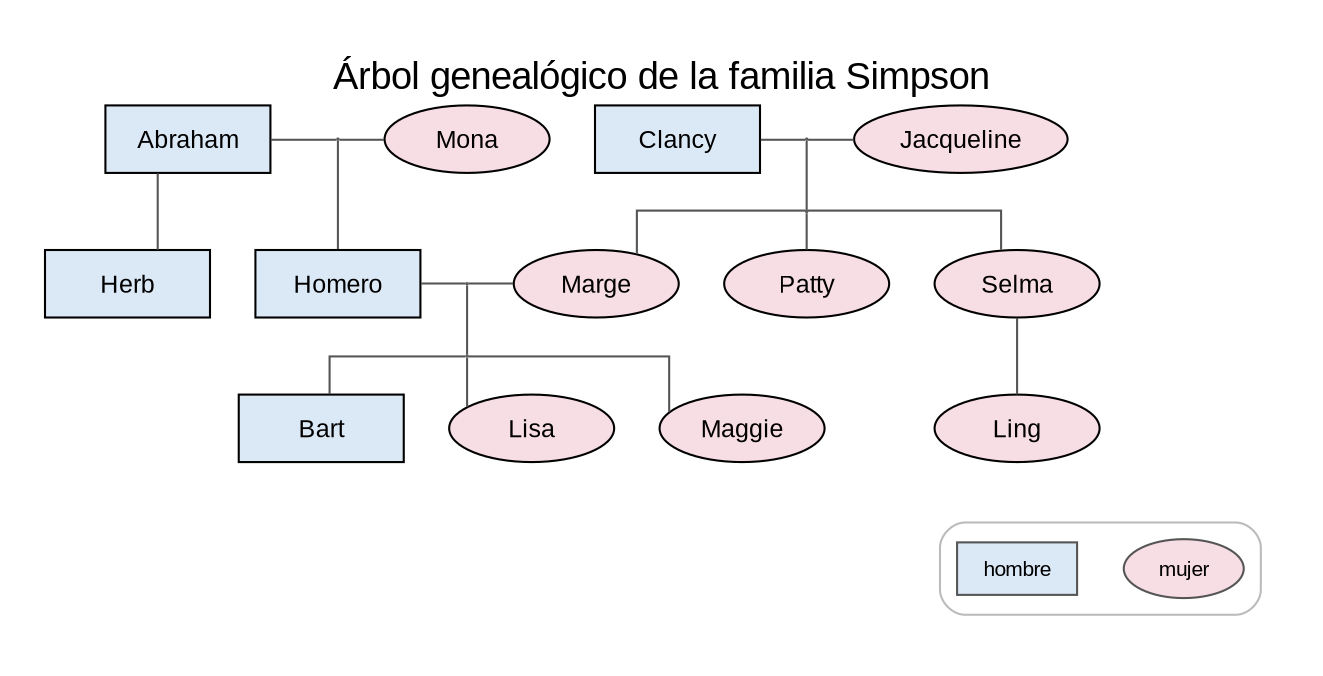
\includegraphics[width=0.95\textwidth]{arbol_genealogico.png}
  \caption{Árbol genealógico de la familia Simpson. Los rectángulos representan
  hombres y las elipses, mujeres.}
  \label{fig:arbol}
\end{figure}

En la figura~\ref{fig:arbol}, cada línea horizontal une a una pareja y de ella
bajan las líneas hacia sus hijos. Herb está unido solo a Abraham y Ling solo a
Selma, porque son los únicos progenitores registrados para ellos.

\noindent\textbf{Consultas y resultados.} Se realizaron las siguientes consultas en
SWI-Prolog:

\begin{lstlisting}
?- progenitor(X, bart).
X = homero ;
X = marge.

?- progenitor(abraham, X).
X = homero ;
X = herb.

?- mujer(ling).
true.

?- hombre(maggie).
false.
\end{lstlisting}

La primera consulta devuelve los dos progenitores de Bart y la segunda, los dos
hijos de Abraham. La última respondió \texttt{false} porque Maggie está
registrada como mujer.

% ------------------------------------------------------------------
\subsection{Ejercicio 1: relaciones \texttt{padre}, \texttt{madre} e \texttt{hijo}}

\noindent\textbf{Enunciado.} Definir las relaciones \texttt{padre(X, Y)}, \texttt{madre(X, Y)}
e \texttt{hijo(X, Y)}, utilizando los hechos \texttt{progenitor/2},
\texttt{hombre/1} y \texttt{mujer/1} del archivo \texttt{familia.pl}.

\noindent\textbf{Razonamiento en lenguaje natural.} Una persona es padre de otra si es su
progenitor y es hombre. Una persona es madre de otra si es su progenitor y es
mujer. Para determinar si X es hijo de Y, se comprueba que Y sea progenitor de X
y que X sea hombre.

\noindent\textbf{Código en Prolog:}

\begin{lstlisting}
% padre(X, Y): X es padre de Y.
padre(X, Y) :-
    progenitor(X, Y),
    hombre(X).

% madre(X, Y): X es madre de Y.
madre(X, Y) :-
    progenitor(X, Y),
    mujer(X).

% hijo(X, Y): X es hijo de Y.
hijo(X, Y) :-
    progenitor(Y, X),
    hombre(X).
\end{lstlisting}

\noindent\textbf{Explicación paso a paso.}
\begin{itemize}
  \item En \texttt{padre}, se comprueba que X sea progenitor de Y y que X sea hombre.
  \item En \texttt{madre}, se comprueba que X sea progenitor de Y y que X sea mujer.
  \item En \texttt{hijo}, se utiliza \texttt{progenitor(Y, X)} porque X es el hijo
  y Y es su progenitor. También se comprueba que X sea hombre.
  \item La coma significa que ambas condiciones deben cumplirse para que la
  relación sea verdadera.
\end{itemize}

\noindent\textbf{Consultas y resultados.} Se realizaron las siguientes consultas en
SWI-Prolog:

\begin{lstlisting}
?- padre(homero, bart).
true.

?- madre(marge, lisa).
true.

?- hijo(bart, homero).
true.

?- hijo(lisa, homero).
false.
\end{lstlisting}

Las primeras tres consultas respondieron \texttt{true}, de acuerdo con los hechos
registrados en el árbol. La última respondió \texttt{false} porque Lisa es mujer y
la regla \texttt{hijo} requiere que el primer argumento sea un hombre.

% ------------------------------------------------------------------
\subsection{Ejercicio 1: relaciones \texttt{hija}, \texttt{abuelo} y \texttt{abuela}}

\noindent\textbf{Enunciado.} Definir las relaciones \texttt{hija(X, Y)},
\texttt{abuelo(X, Y)} y \texttt{abuela(X, Y)}, utilizando los hechos
\texttt{progenitor/2}, \texttt{hombre/1} y \texttt{mujer/1} del archivo
\texttt{familia.pl}.

\noindent\textbf{Razonamiento en lenguaje natural.} X es hija de Y si Y es progenitor de X
y X es mujer. X es abuelo de Y si X es progenitor de alguno de los progenitores de
Y y X es hombre. La relación abuela se define de la misma forma, pero X debe ser
mujer. Por ejemplo, Clancy es progenitor de Selma y Selma es progenitora de Ling,
por lo que Clancy es abuelo de Ling.

\noindent\textbf{Código en Prolog:} Las reglas se agregaron al archivo \texttt{familia.pl},
después de las reglas anteriores.

\begin{lstlisting}
% hija(X, Y): X es hija de Y (hija primero, progenitor despues).
hija(X, Y) :-
    progenitor(Y, X),
    mujer(X).

% abuelo(X, Y): X es abuelo de Y por cualquiera de sus progenitores.
abuelo(X, Y) :-
    progenitor(X, Z),
    progenitor(Z, Y),
    hombre(X).

% abuela(X, Y): X es abuela de Y por cualquiera de sus progenitores.
abuela(X, Y) :-
    progenitor(X, Z),
    progenitor(Z, Y),
    mujer(X).
\end{lstlisting}

\noindent\textbf{Explicación paso a paso.}
\begin{itemize}
  \item En \texttt{hija}, se utiliza \texttt{progenitor(Y, X)} porque Y es el
  progenitor y X es la hija. Después, \texttt{mujer(X)} comprueba que X sea mujer.
  \item En \texttt{abuelo}, \texttt{progenitor(X, Z)} y \texttt{progenitor(Z, Y)}
  buscan una persona Z que sea hija o hijo de X y, a la vez, progenitor de Y. Z
  representa la generación intermedia.
  \item Como Z puede ser el padre o la madre de Y, la regla encuentra a los abuelos
  de ambos lados de la familia.
  \item \texttt{hombre(X)} en \texttt{abuelo} y \texttt{mujer(X)} en
  \texttt{abuela} distinguen entre abuelo y abuela.
\end{itemize}

\noindent\textbf{Consultas y resultados.} Se realizaron las siguientes consultas en
SWI-Prolog:

\begin{lstlisting}
?- hija(lisa, homero).
true.

?- hija(bart, homero).
false.

?- abuelo(abraham, bart).
true ;
false.

?- abuela(jacqueline, ling).
true.

?- abuelo(X, ling).
X = clancy ;
false.

?- abuela(mona, ling).
false.
\end{lstlisting}

Cuando Prolog responde \texttt{true ;} seguido de \texttt{false}, significa que
encontró la respuesta y que, al pedirle otra con \texttt{;}, ya no encontró otra
forma de demostrarla. La consulta \texttt{hija(bart, homero)} respondió
\texttt{false} porque Bart es hombre, y \texttt{abuela(mona, ling)} respondió
\texttt{false} porque Mona es abuela por el lado de Homero, mientras que Ling es
hija de Selma.

Además, con \texttt{setof/3} se obtuvieron todas las parejas de cada relación:

\begin{center}
\begin{tabular}{|p{4cm}|p{2.2cm}|p{6cm}|}
\hline
\textbf{Consulta} & \textbf{Resultado} & \textbf{Explicación} \\
\hline
\texttt{hija(X, Y)} & 11 parejas & Lisa y Maggie con Homero y Marge (4); Marge,
Patty y Selma con Clancy y Jacqueline (6); Ling con Selma (1). \\
\hline
\texttt{abuelo(X, Y)} & 7 parejas & Abraham es abuelo de Bart, Lisa y Maggie;
Clancy es abuelo de Bart, Lisa, Maggie y Ling. \\
\hline
\texttt{abuela(X, Y)} & 7 parejas & Mona es abuela de Bart, Lisa y Maggie;
Jacqueline es abuela de Bart, Lisa, Maggie y Ling. \\
\hline
\end{tabular}
\end{center}

% ------------------------------------------------------------------
\subsection{Ejercicio 1: relaciones \texttt{hermano}, \texttt{hermana} y \texttt{tio}}

\noindent\textbf{Enunciado.} Definir en Prolog, sobre el árbol genealógico de la familia
Simpson, las relaciones \texttt{hermano(X, Y)}, \texttt{hermana(X, Y)} y
\texttt{tio(X, Y)}, donde X es hermano, hermana o tío de Y, respectivamente. Las
tres se construyen a partir de los hechos \texttt{hombre/1}, \texttt{mujer/1} y
\texttt{progenitor/2}, que se cargan desde el archivo \texttt{familia.pl}. Las
reglas se escribieron en el archivo \texttt{hermanos\_tios.pl}.

\noindent\textbf{Razonamiento en lenguaje natural.} Dos personas son hermanos cuando son
distintas y tienen al menos un progenitor en común. Si X es hombre, X es hermano
de Y, y si X es mujer, X es hermana de Y. Por otro lado, X es tío de Y cuando X es
hermano de alguno de los progenitores de Y. Por ejemplo, Herb y Homero tienen como
progenitor a Abraham, por lo que son hermanos; como Homero es progenitor de Bart,
Herb es tío de Bart.

\noindent\textbf{Código en Prolog:}

\begin{figure}[H]
  \centering
  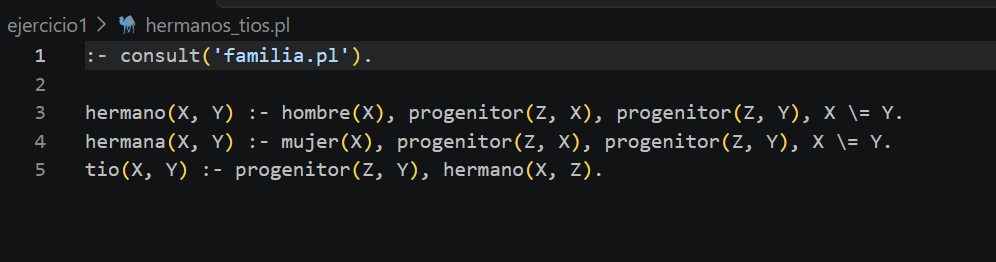
\includegraphics[width=0.95\textwidth]{hermanos_tios_codigo.png}
  \caption{Reglas \texttt{hermano}, \texttt{hermana} y \texttt{tio} en el archivo
  \texttt{hermanos\_tios.pl}.}
  \label{fig:hermanos_codigo}
\end{figure}

\noindent\textbf{Explicación paso a paso.}
\begin{itemize}
  \item \texttt{:- consult('familia.pl').} carga los hechos \texttt{hombre/1},
  \texttt{mujer/1} y \texttt{progenitor/2} del árbol genealógico, para que las
  reglas puedan utilizarlos.
  \item \texttt{hombre(X)} comprueba que X sea hombre. En \texttt{hermana} se usa
  \texttt{mujer(X)}, que comprueba que X sea mujer.
  \item \texttt{progenitor(Z, X), progenitor(Z, Y)} busca un Z que sea progenitor
  de X y de Y al mismo tiempo, es decir, un progenitor en común.
  \item \texttt{X \textbackslash= Y} exige que X y Y sean personas distintas. Sin
  esta condición, cada persona resultaría hermano o hermana de sí misma.
  \item En \texttt{tio}, \texttt{progenitor(Z, Y)} toma un progenitor Z de Y, y
  \texttt{hermano(X, Z)} comprueba que X sea hermano de Z.
\end{itemize}

\noindent\textbf{Respuestas repetidas.} Si dos hermanos comparten a sus dos progenitores,
la misma pareja se obtiene una vez por cada progenitor en común. Por ejemplo, Bart
y Lisa comparten a Homero y a Marge. Para mostrar cada resultado una sola vez se
utilizó \texttt{setof/3}, que además ordena los resultados y elimina los repetidos.

\noindent\textbf{Consultas y resultados.} En la siguiente tabla se resumen las consultas
realizadas.

\begin{center}
\begin{tabular}{|p{4cm}|p{2.2cm}|p{6cm}|}
\hline
\textbf{Consulta} & \textbf{Resultado} & \textbf{Explicación} \\
\hline
\texttt{hermano(X, Y)} & 4 parejas & Bart es hermano de Lisa y de Maggie; Herb y
Homero son hermanos porque ambos tienen a Abraham como progenitor. \\
\hline
\texttt{hermana(X, Y)} & 10 parejas & Marge, Patty y Selma son hermanas entre sí
(6 parejas); Lisa y Maggie son hermanas entre sí y de Bart (4 parejas). \\
\hline
\texttt{tio(X, Y)} & 3 parejas & Herb es tío de Bart, Lisa y Maggie. \\
\hline
\texttt{tio(herb, bart)} & \texttt{true} & Herb es hermano de Homero, que es
progenitor de Bart. \\
\hline
\end{tabular}
\end{center}

\noindent\textbf{Comprobación en Prolog.}

\begin{figure}[H]
  \centering
  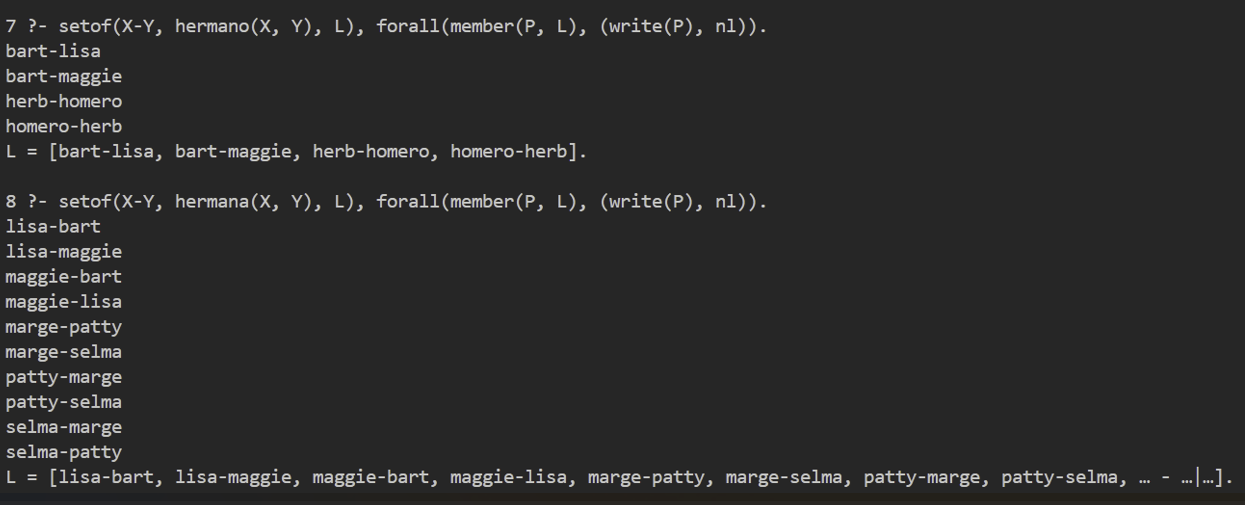
\includegraphics[width=0.95\textwidth]{consulta_hermanos.png}
  \caption{Resultado de las consultas \texttt{hermano(X, Y)} y
  \texttt{hermana(X, Y)} en Prolog.}
  \label{fig:hermanos}
\end{figure}

En la figura~\ref{fig:hermanos}, la consulta \texttt{hermano(X, Y)} devolvió 4
parejas: \texttt{bart-lisa}, \texttt{bart-maggie}, \texttt{herb-homero} y
\texttt{homero-herb}. La consulta \texttt{hermana(X, Y)} devolvió 10 parejas, que
corresponden a las hermanas del árbol: Marge, Patty y Selma entre sí, y Lisa y
Maggie entre sí y con Bart.

\begin{figure}[H]
  \centering
  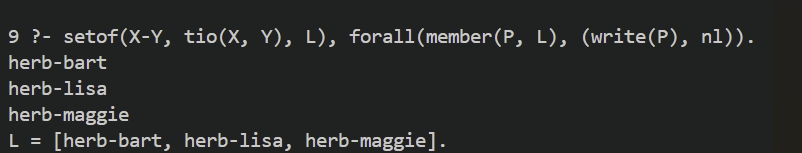
\includegraphics[width=0.7\textwidth]{consulta_tio.png}
  \caption{Resultado de la consulta \texttt{tio(X, Y)} en Prolog.}
  \label{fig:tio}
\end{figure}

En la figura~\ref{fig:tio}, la consulta devolvió 3 parejas: \texttt{herb-bart},
\texttt{herb-lisa} y \texttt{herb-maggie}.

\begin{figure}[H]
  \centering
  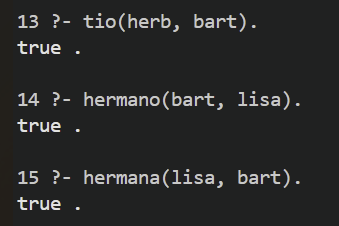
\includegraphics[width=0.4\textwidth]{consultas_verificacion.png}
  \caption{Consultas de verificación en Prolog.}
  \label{fig:verificacion}
\end{figure}

En la figura~\ref{fig:verificacion}, las tres consultas respondieron
\texttt{true}. Esto indica que Prolog logró demostrarlas con los hechos del árbol:
Herb es hermano de Homero y Homero es progenitor de Bart, y Bart y Lisa comparten a
Homero como progenitor.

\noindent\textbf{Observación.} Herb es el único tío del árbol. Clancy solo tiene hijas
(Marge, Patty y Selma), por lo que de ese lado no hay tíos hombres y Ling tiene
tías pero no tíos.

% ------------------------------------------------------------------
\subsection{Ejercicio 1: relaciones \texttt{tia}, \texttt{sobrino} y \texttt{sobrina}}

\noindent\textbf{Enunciado.} Definir las relaciones \texttt{tia(X, Y)},
\texttt{sobrino(X, Y)} y \texttt{sobrina(X, Y)}, donde X es tía, sobrino o sobrina
de Y, respectivamente. Las reglas se escribieron en el archivo
\texttt{tias\_sobrinos.pl}, que carga \texttt{hermanos\_tios.pl} para utilizar las
relaciones \texttt{hermana} y \texttt{tio} definidas anteriormente.

\noindent\textbf{Razonamiento en lenguaje natural.} X es tía de Y cuando X es hermana de
alguno de los progenitores de Y. X es sobrino de Y cuando X es hombre y Y es su tío
o su tía. La relación sobrina se define de la misma forma, pero X debe ser mujer.
Por ejemplo, Patty es hermana de Marge y Marge es progenitora de Bart, por lo que
Patty es tía de Bart y Bart es sobrino de Patty.

\noindent\textbf{Código en Prolog:}

\begin{lstlisting}
:- consult('hermanos_tios.pl').

% tia(X, Y): X es tia de Y.
tia(X, Y) :-
    progenitor(Z, Y),
    hermana(X, Z).

% sobrino(X, Y): X es sobrino de Y.
sobrino(X, Y) :-
    hombre(X),
    tio(Y, X).
sobrino(X, Y) :-
    hombre(X),
    tia(Y, X).

% sobrina(X, Y): X es sobrina de Y.
sobrina(X, Y) :-
    mujer(X),
    tio(Y, X).
sobrina(X, Y) :-
    mujer(X),
    tia(Y, X).
\end{lstlisting}

\noindent\textbf{Explicación paso a paso.}
\begin{itemize}
  \item \texttt{:- consult('hermanos\_tios.pl').} carga las reglas
  \texttt{hermano}, \texttt{hermana} y \texttt{tio}, y con ellas los hechos de
  \texttt{familia.pl}.
  \item \texttt{tia} sigue la misma idea que \texttt{tio}: \texttt{progenitor(Z, Y)}
  toma un progenitor Z de Y, y \texttt{hermana(X, Z)} comprueba que X sea hermana
  de Z.
  \item \texttt{sobrino} tiene dos reglas: la primera se cumple cuando Y es tío de X
  y la segunda, cuando Y es tía de X. Prolog prueba las dos en orden. La relación
  \texttt{sobrina} funciona igual.
  \item \texttt{hombre(X)} en \texttt{sobrino} y \texttt{mujer(X)} en
  \texttt{sobrina} distinguen entre sobrino y sobrina.
  \item Estas relaciones son inversas a las de tío y tía: si Patty es tía de Bart,
  entonces Bart es sobrino de Patty.
\end{itemize}

\noindent\textbf{Respuestas repetidas.} Marge, Patty y Selma comparten a sus dos
progenitores, por lo que \texttt{hermana} devuelve cada una de esas parejas dos
veces y \texttt{tia} conserva esa repetición. Por eso, en la consulta
\texttt{tia(X, ling)}, Marge y Patty aparecen dos veces cada una. Al igual que en
la sección anterior, para contar los resultados sin repetir se utilizó
\texttt{setof/3}.

\noindent\textbf{Consultas y resultados.} Se realizaron las siguientes consultas en
SWI-Prolog:

\begin{lstlisting}
?- tia(patty, bart).
true ;
true.

?- tia(X, ling).
X = marge ;
X = marge ;
X = patty ;
X = patty ;
false.

?- sobrino(bart, herb).
true ;
false.

?- sobrina(ling, marge).
true ;
true.

?- tio(homero, ling).
false.
\end{lstlisting}

\begin{center}
\begin{tabular}{|p{4cm}|p{2.2cm}|p{6cm}|}
\hline
\textbf{Consulta} & \textbf{Resultado} & \textbf{Explicación} \\
\hline
\texttt{tia(X, Y)} & 8 parejas & Patty y Selma son tías de Bart, Lisa y Maggie;
Marge y Patty son tías de Ling. \\
\hline
\texttt{sobrino(X, Y)} & 3 parejas & Bart es sobrino de Herb, Patty y Selma. \\
\hline
\texttt{sobrina(X, Y)} & 8 parejas & Lisa y Maggie son sobrinas de Herb, Patty y
Selma; Ling es sobrina de Marge y Patty. \\
\hline
\end{tabular}
\end{center}

\noindent\textbf{Observación.} La consulta \texttt{tio(homero, ling)} respondió
\texttt{false}. Homero es esposo de Marge, que es hermana de Selma, pero no es
hermano de Selma. Como el árbol solo registra relaciones de progenitor y no
matrimonios, las reglas consideran únicamente a los tíos y tías de sangre.

% ------------------------------------------------------------------
\subsection{Ejercicio 2: hechos del grafo}

\noindent\textbf{Enunciado.} Representar en Prolog el grafo dirigido con vértices
$\{a, b, c, d\}$ y arcos $\{(a, b),\allowbreak (a, c),\allowbreak (a, d),\allowbreak (c, d)\}$.

\noindent\textbf{Razonamiento en lenguaje natural.} Cada arco del grafo es una flecha que va
de un vértice a otro. Se representa con un hecho \texttt{arco(X, Y)}, que indica
que existe un arco desde X hasta Y. Los vértices no necesitan hechos propios,
porque aparecen dentro de los arcos.

\noindent\textbf{Código en Prolog:} Los hechos se escribieron al inicio del archivo
\texttt{grafo.pl}.

\begin{lstlisting}
% Ejercicio 2: grafo dirigido ({a,b,c,d}, {(a,b),(a,c),(a,d),(c,d)})

% arco(X, Y): existe una arista dirigida de X a Y.
arco(a, b).
arco(a, c).
arco(a, d).
arco(c, d).
\end{lstlisting}

\noindent\textbf{Explicación paso a paso.}
\begin{itemize}
  \item Hay un hecho por cada arco del grafo, en el mismo orden del enunciado.
  \item El grafo es dirigido, por lo que \texttt{arco(a, b)} no implica que exista
  un arco de b hacia a.
  \item De los vértices b y d no sale ningún arco. Solo reciben arcos.
  \item Prolog revisa los hechos de arriba hacia abajo, por lo que este orden
  determina el orden de las soluciones y de las ramas del árbol de búsqueda.
\end{itemize}

\noindent\textbf{Consultas y resultados.} Se realizaron las siguientes consultas en
SWI-Prolog:

\begin{lstlisting}
?- arco(a, X).
X = b ;
X = c ;
X = d.

?- arco(X, d).
X = a ;
X = c.

?- arco(d, X).
false.
\end{lstlisting}

La primera consulta devuelve los tres vértices a los que se llega desde a, en el
orden en que están escritos los hechos. La segunda devuelve los vértices que tienen
un arco directo hacia d. La última respondió \texttt{false} porque de d no sale
ningún arco.

% ------------------------------------------------------------------
\subsection{Ejercicio 2: definición del predicado \texttt{camino}}

\noindent\textbf{Enunciado.} Definir el predicado \texttt{camino/3} para encontrar caminos
en el grafo dirigido con vértices $\{a, b, c, d\}$ y arcos
$\{(a, b), (a, c), (a, d), (c, d)\}$.

\noindent\textbf{Razonamiento en lenguaje natural.} Existe un camino entre dos vértices si
hay un arco directo entre ellos, o si se puede avanzar a un vértice intermedio y
continuar desde allí hasta el destino. Estas posibilidades se representan con un
caso base y un caso recursivo.

\noindent\textbf{Código en Prolog:} Las siguientes reglas se agregaron al archivo
\texttt{grafo.pl}, después de los hechos \texttt{arco/2}.

\begin{lstlisting}
% camino(X, Y, C): C es un camino desde X hasta Y.

% Caso base: hay un arco directo.
camino(X, Y, [X, Y]) :-
    arco(X, Y).

% Caso recursivo: pasar por un vertice intermedio Z.
camino(X, Y, [X | Resto]) :-
    arco(X, Z),
    camino(Z, Y, Resto).
\end{lstlisting}

\noindent\textbf{Explicación paso a paso.}
\begin{itemize}
  \item En \texttt{camino(X, Y, C)}, X es el vértice inicial, Y es el destino y C
  es la lista de vértices que forman el camino.
  \item El caso base comprueba si existe \texttt{arco(X, Y)}. Si existe, el camino
  es la lista \texttt{[X, Y]}.
  \item El caso recursivo busca un arco desde X hasta un vértice intermedio Z.
  Luego llama nuevamente a \texttt{camino} para buscar cómo llegar desde Z hasta Y.
  \item En \texttt{[X | Resto]}, X es el primer elemento de la lista y
  \texttt{Resto} contiene el camino encontrado desde Z hasta el destino.
\end{itemize}

\noindent\textbf{Ejemplo.} Para construir el camino \texttt{[a,c,d]}, la regla recursiva
utiliza el arco de a hacia c. Después busca un camino de c hacia d. Como existe un
arco directo entre estos vértices, el caso base obtiene \texttt{[c,d]}.
Finalmente, se coloca a al inicio de la lista y se forma \texttt{[a,c,d]}.

\noindent\textbf{Observación.} Esta definición encuentra caminos de al menos un arco y es
suficiente para el grafo de la tarea, que no contiene ciclos. Las consultas y sus
resultados se presentan en el siguiente apartado.

% ------------------------------------------------------------------
\subsection{Ejercicio 2: ejecución de la consulta \texttt{camino(X, d, Y)}}
\label{sec:ejecucion}

\noindent\textbf{Enunciado.} Se tiene el grafo dirigido
$(\{a, b, c, d\}, \{(a, b), (a, c), (a, d), (c, d)\})$, cuyos arcos y el predicado
\texttt{camino} se encuentran en el archivo \texttt{grafo.pl}. Se debe ejecutar la
consulta \texttt{camino(X, d, Y)}, donde X es un vértice de inicio y Y es el
camino, y obtener todas sus soluciones.

\noindent\textbf{Consulta en Prolog:}

\begin{lstlisting}
camino(X, d, Y).
\end{lstlisting}

Después de cada respuesta se pulsa \texttt{;} para que Prolog retroceda y busque
otra solución, hasta que responde \texttt{false}. Para ver todas las soluciones
juntas se utilizó:

\begin{lstlisting}
forall(camino(X, d, Y), (write(X-Y), nl)).
\end{lstlisting}

\noindent\textbf{Resultados.} Prolog devolvió tres soluciones:

\begin{center}
\begin{tabular}{|c|c|p{6.5cm}|}
\hline
\textbf{X} & \textbf{Y} & \textbf{Interpretación} \\
\hline
a & [a, d] & Desde a se llega a d directamente, por el arco $(a, d)$. \\
\hline
c & [c, d] & Desde c se llega a d directamente, por el arco $(c, d)$. \\
\hline
a & [a, c, d] & Desde a se llega a c y desde c se llega a d. \\
\hline
\end{tabular}
\end{center}

\noindent\textbf{Comprobación en Prolog.}

\begin{figure}[H]
  \centering
  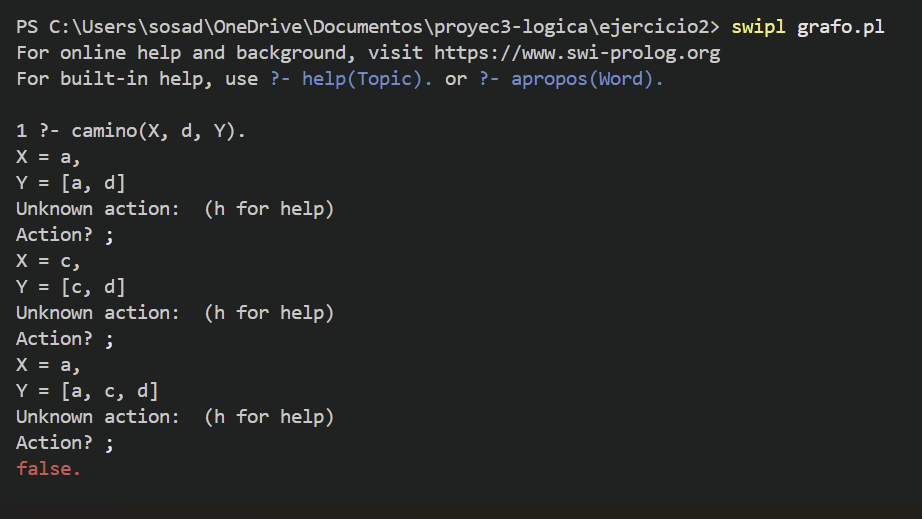
\includegraphics[width=0.7\textwidth]{camino_una_por_una.png}
  \caption{Soluciones de \texttt{camino(X, d, Y)} obtenidas una por una.}
  \label{fig:camino_una}
\end{figure}

En la figura~\ref{fig:camino_una}, Prolog muestra las tres soluciones y, después
de la tercera, responde \texttt{false}, lo que indica que no existen más caminos
que terminen en \texttt{d}.

\begin{figure}[H]
  \centering
  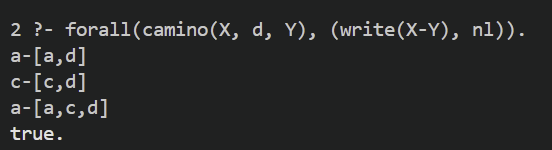
\includegraphics[width=0.55\textwidth]{camino_forall.png}
  \caption{Todas las soluciones de \texttt{camino(X, d, Y)} en una sola consulta.}
  \label{fig:camino_forall}
\end{figure}

En la figura~\ref{fig:camino_forall}, las tres soluciones se muestran juntas, una
por línea.

\noindent\textbf{Observación.} Los vértices \texttt{b} y \texttt{d} no aparecen como inicio
de ningún camino hacia \texttt{d}, porque de ellos no sale ningún arco. Las tres
soluciones obtenidas coinciden con las tres hojas de éxito del árbol de búsqueda
de la consulta.

% ------------------------------------------------------------------
\subsection{Ejercicio 2: árbol de búsqueda de \texttt{camino(X, d, Y)}}

\noindent\textbf{Enunciado.} Graficar el árbol de búsqueda que recorre Prolog para resolver
la consulta \texttt{camino(X, d, Y)}, utilizando un programa.

\noindent\textbf{Programa utilizado.} El árbol se generó con el programa
\texttt{generar\_arbol.py}, escrito en Python, en lugar de SldDraw, que el
enunciado menciona como ejemplo. El programa lee las reglas y los hechos del
archivo \texttt{grafo.pl} y recorre la búsqueda en el mismo orden que Prolog:
prueba primero el caso base y después el caso recursivo, y revisa los hechos
\texttt{arco/2} de arriba hacia abajo. El resultado es la imagen
\texttt{arbol\_busqueda.png}, que se muestra en la figura~\ref{fig:arbol_busqueda}.

\noindent\textbf{Cómo leer el árbol.}
\begin{itemize}
  \item La raíz es la consulta \texttt{camino(X,d,Y)}. Cada nodo muestra los
  objetivos que Prolog todavía debe demostrar.
  \item Cada rama corresponde a una regla o a un hecho que coincide con el
  objetivo. La etiqueta indica qué caso se usó (\texttt{base} o \texttt{rec.}) y
  qué valores tomaron las variables.
  \item Las hojas verdes son éxitos: ya no quedan objetivos y se obtiene una
  solución. Las hojas rojas son fallos: ningún hecho coincide con el objetivo.
  \item \texttt{Z1}, \texttt{R1}, \texttt{Z2}, \texttt{R2} y \texttt{Z3},
  \texttt{R3} son nombres nuevos que reciben las variables cada vez que Prolog
  vuelve a usar la regla recursiva, para no confundirlas con las de la llamada
  anterior.
\end{itemize}

\noindent\textbf{Explicación paso a paso.} Para recorrer el árbol, Prolog utiliza dos
mecanismos. El primero es la unificación, que consiste en hacer coincidir un
objetivo con un hecho o con el inicio de una regla, asignando valores a las
variables. El segundo es el retroceso (\emph{backtracking}), que consiste en
regresar a la última decisión en la que quedaba otra opción, ya sea porque una
rama falló o porque se pidió otra solución con \texttt{;}.

\begin{enumerate}
  \item Prolog toma el objetivo \texttt{camino(X, d, Y)} y lo unifica con el caso
  base, \texttt{camino(X, Y, [X, Y])}. Para que coincidan, Y debe ser la lista
  \texttt{[X, d]}, y el nuevo objetivo es \texttt{arco(X, d)}.
  \item Prolog revisa los hechos \texttt{arco/2} en orden. \texttt{arco(a, b)} y
  \texttt{arco(a, c)} no coinciden, porque su segundo vértice no es d.
  \texttt{arco(a, d)} sí coincide con X = a, así que se obtiene la primera
  solución: X = a, Y = [a, d].
  \item Al pulsar \texttt{;}, Prolog retrocede y sigue revisando los hechos desde
  donde se quedó. \texttt{arco(c, d)} coincide con X = c y se obtiene la segunda
  solución: X = c, Y = [c, d].
  \item Ya no quedan hechos que coincidan con \texttt{arco(X, d)}, así que Prolog
  retrocede hasta la consulta inicial y prueba el caso recursivo. Ahora
  Y = [X | R1] y los objetivos pendientes son \texttt{arco(X, Z1)} y
  \texttt{camino(Z1, d, R1)}.
  \item El primer hecho que coincide con \texttt{arco(X, Z1)} es \texttt{arco(a, b)},
  con X = a y Z1 = b. Prolog debe demostrar \texttt{camino(b, d, R1)}. El caso base
  necesita \texttt{arco(b, d)} y el caso recursivo necesita un arco que salga de b.
  Ninguno existe, por lo que las dos ramas fallan y Prolog retrocede.
  \item El siguiente hecho es \texttt{arco(a, c)}, con Z1 = c. Para
  \texttt{camino(c, d, R1)}, el caso base encuentra \texttt{arco(c, d)}, así que
  R1 = [c, d] y, por lo tanto, Y = [a, c, d]. Esta es la tercera solución.
  \item Al pulsar \texttt{;} de nuevo, Prolog prueba el caso recursivo de
  \texttt{camino(c, d, R1)}. Usa \texttt{arco(c, d)} con Z2 = d y debe demostrar
  \texttt{camino(d, d, R2)}. Como de d no sale ningún arco, ni el caso base ni el
  recursivo encuentran hechos y la rama falla.
  \item Prolog retrocede a \texttt{arco(X, Z1)} y usa \texttt{arco(a, d)}, con
  Z1 = d. Otra vez debe demostrar \texttt{camino(d, d, R1)}, que falla por la misma
  razón.
  \item Por último, usa \texttt{arco(c, d)}, con X = c y Z1 = d. Se repite el
  objetivo \texttt{camino(d, d, R1)}, que también falla.
  \item No quedan opciones por probar en ninguna rama, así que Prolog responde
  \texttt{false}.
\end{enumerate}

En total, el árbol tiene tres hojas de éxito, que coinciden con las tres
soluciones obtenidas en la sección~\ref{sec:ejecucion}, y ocho hojas de fallo.

\noindent\textbf{Observación.} El orden de los hechos en \texttt{grafo.pl} determina el
orden de las soluciones. Por ejemplo, si \texttt{arco(c, d)} estuviera escrito
antes que \texttt{arco(a, d)}, la primera solución sería X = c, Y = [c, d].

\begin{landscape}
\begin{figure}[H]
  \centering
  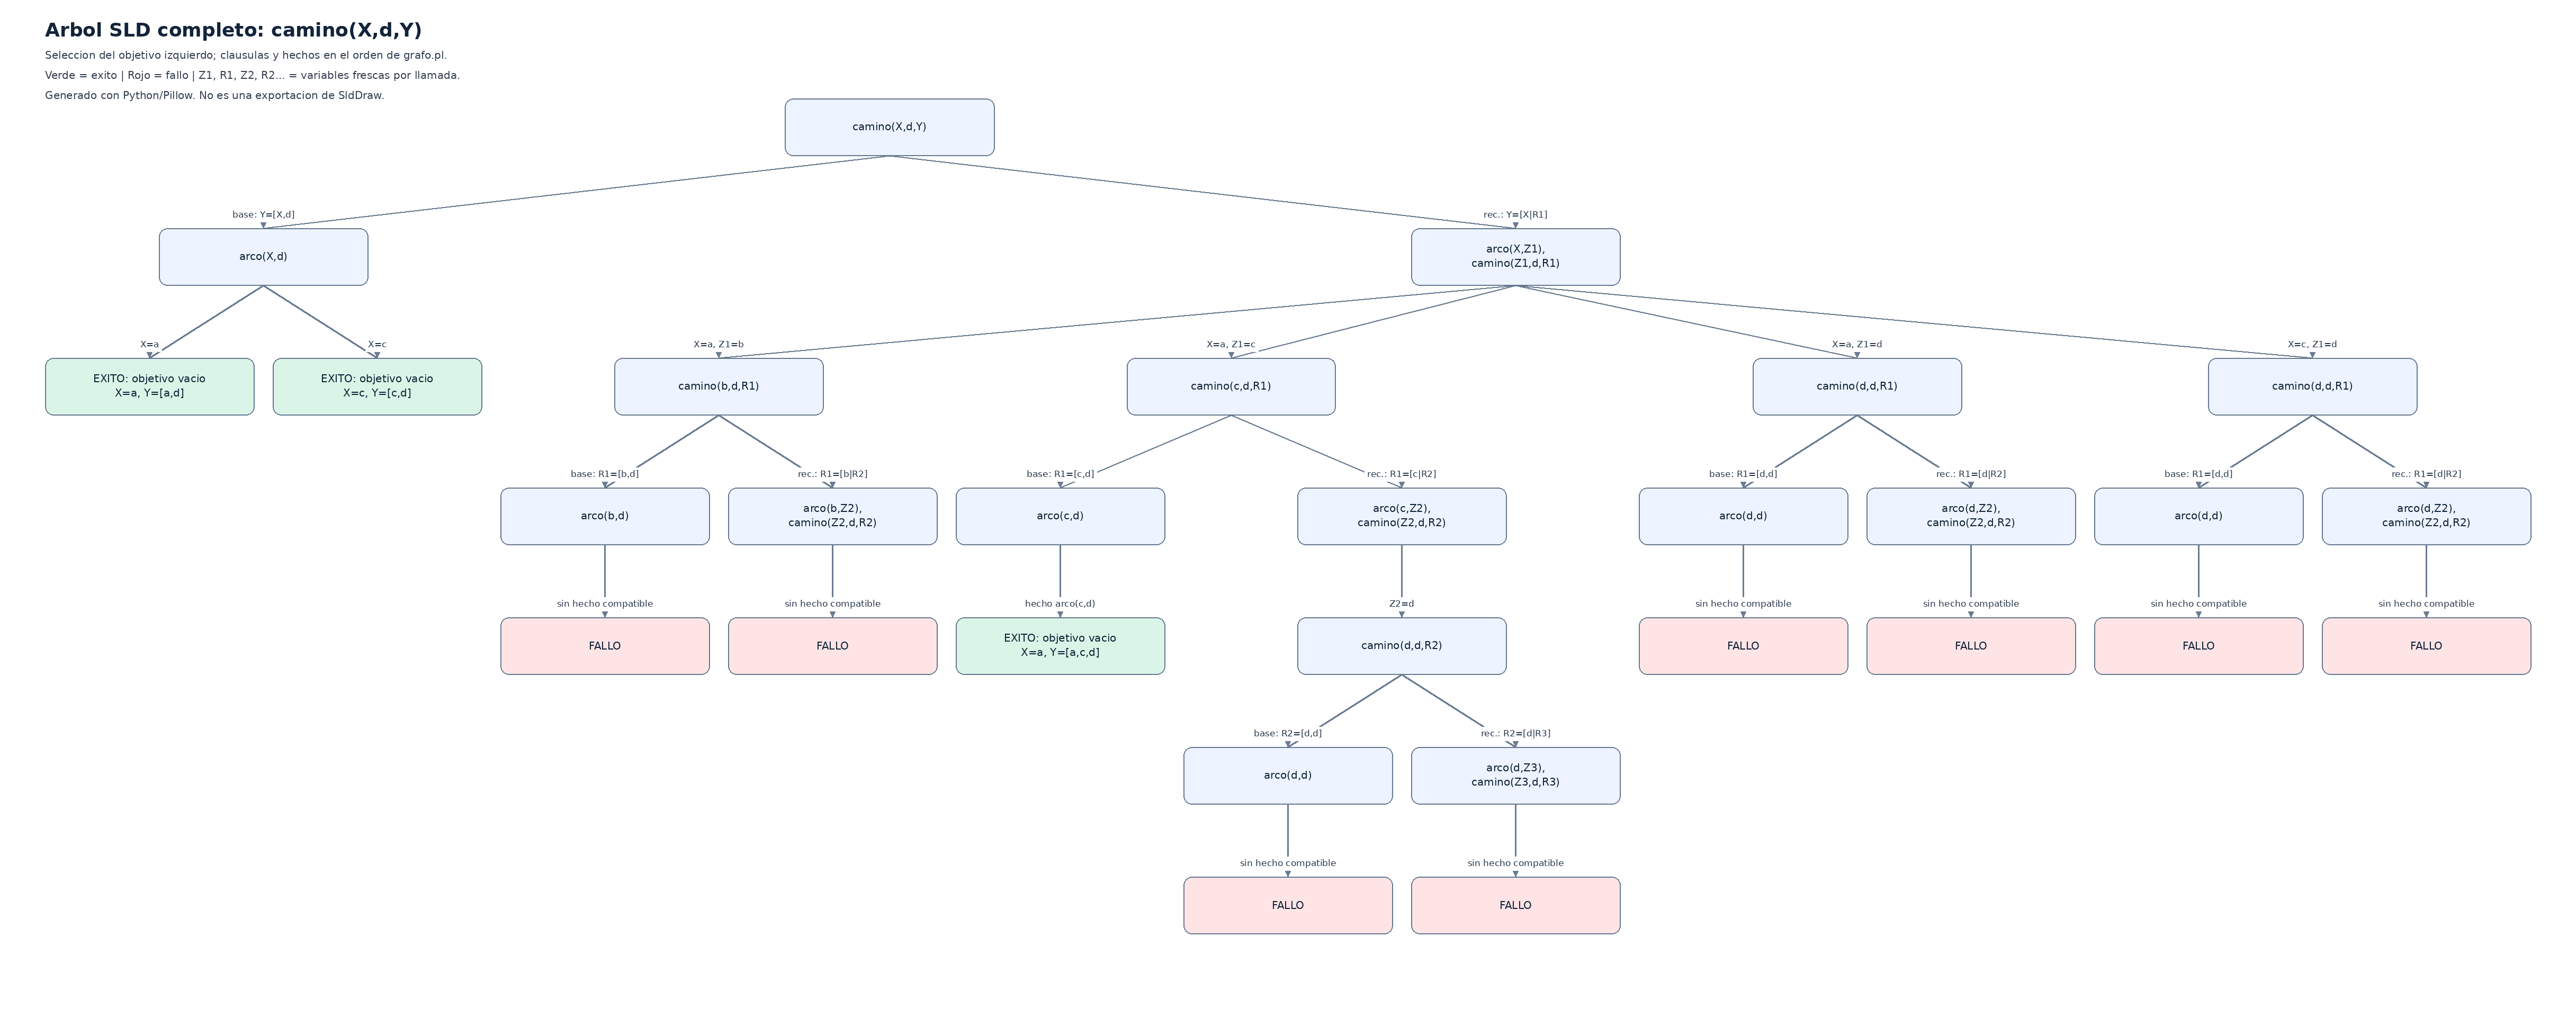
\includegraphics[width=\linewidth]{arbol_busqueda.png}
  \caption{Árbol de búsqueda de la consulta \texttt{camino(X, d, Y)}.}
  \label{fig:arbol_busqueda}
\end{figure}
\end{landscape}

% ------------------------------------------------------------------
\section{Archivos entregados}

\begin{center}
\begin{tabular}{|p{6.6cm}|p{8.4cm}|}
\hline
\textbf{Archivo} & \textbf{Contenido} \\
\hline
\texttt{ejercicio1/familia.pl} & Hechos \texttt{hombre}, \texttt{mujer} y
\texttt{progenitor}, y reglas \texttt{padre}, \texttt{madre}, \texttt{hijo},
\texttt{hija}, \texttt{abuelo} y \texttt{abuela}. \\
\hline
\texttt{ejercicio1/hermanos\_tios.pl} & Reglas \texttt{hermano}, \texttt{hermana}
y \texttt{tio}. \\
\hline
\texttt{ejercicio1/tias\_sobrinos.pl} & Reglas \texttt{tia}, \texttt{sobrino} y
\texttt{sobrina}. \\
\hline
\texttt{ejercicio1/arbol.png} & Representación gráfica del árbol genealógico. \\
\hline
\texttt{ejercicio1/arbol.dot} & Archivo con el que se genera el dibujo del árbol
genealógico. \\
\hline
\texttt{ejercicio2/grafo.pl} & Hechos \texttt{arco} y predicado \texttt{camino}. \\
\hline
\texttt{ejercicio2/consulta\_camino.pl} & Consulta \texttt{camino(X, d, Y)}. \\
\hline
\texttt{ejercicio2/generar\_arbol.py} & Programa que genera el árbol de búsqueda. \\
\hline
\texttt{ejercicio2/arbol\_busqueda.png} & Árbol de búsqueda de la consulta
\texttt{camino(X, d, Y)}. \\
\hline
\texttt{ejercicio2/arbol\_busqueda.dot} & Descripción del árbol de búsqueda en
formato DOT. \\
\hline
\end{tabular}
\end{center}

Para utilizar todas las relaciones del Ejercicio 1 basta con cargar
\texttt{tias\_sobrinos.pl} en SWI-Prolog, ya que este archivo carga
\texttt{hermanos\_tios.pl} y, a su vez, \texttt{familia.pl}.

\end{document}
